\chapter{Text Recognition: Methods and Application Case Study}
\clearpage
%\begin{comment}
    
  
\section{Introduction}
\vspace{-0.5cm}

%In today's digital age, extracting meaningful information from visual data has become an important component of many intelligent systems. Text recognition, in particular, plays a crucial role in the context of unstructured visual content and structured, machine-readable data. Whether it is digitizing historical manuscripts, automating administrative workflows, or enabling smart healthcare applications. \textcolor{red}{redo this paragraph}


In an increasingly digital world, the ability to extract meaningful information from visual content has become essential across many fields. Text recognition, in particular, serves as a key technology for converting written or printed text within images into machine-readable formats. It enables a wide range of applications—from digitizing historical documents and automating data entry to supporting intelligent healthcare systems and assistive technologies. As the volume of visual data grows, the demand for accurate and efficient text recognition methods continues to rise.


This chapter explores the fundamental key concepts in the field of text recognition. It begins by defining what text recognition is and how it has evolved from traditional rule-based systems to modern deep learning-based approaches. The chapter also covers the essential image processing steps that prepare images for recognition, explains how Optical Character Recognition (OCR) works, and introduces several widely used open-source OCR engines, including Tesseract, EasyOCR, and TrOCR.
Additionally, the chapter outlines a typical OCR pipeline—from pre-processing and text detection to recognition and post-processing—providing a comprehensive overview of how raw image data is transformed into actionable text. A particular focus is given to practical applications, especially in domains such as healthcare and document analysis, where accurate text recognition can have a significant impact.%corrected
\vspace{-0.5cm}
\section{What is Text Recognition?}
Text Recognition has been a crucial part of Artificial Intelligence throughout the years. It enables machines to extract, interpret, and process textual information from images and scanned documents. This technology can be applied in various applications such as document digitization, automation of data entries in intelligent search systems like a camera-based analysis of text and documents \cite{liang2005camera}, and an NLP System for information extraction from electronic medical records \cite{savova2010mayo}. At first, text recognition relied on rule-based techniques and feature extraction. However, the recent advancements in Deep Learning and Neural Networks have significantly improved the accuracy and adaptability. Techniques such as Optical Character Recognition (OCR), Automatic Speech Recognition (ASR), and Handwritten Text Recognition (HTR) have shown promising progress in their application and are now more reliably used throughout different fields and domains \cite{alkendi2024advancements, mori1992historical, karpagavalli2016review}. %corrected
\vspace{-0.5cm}
\begin{figure}[H]
    \centering
    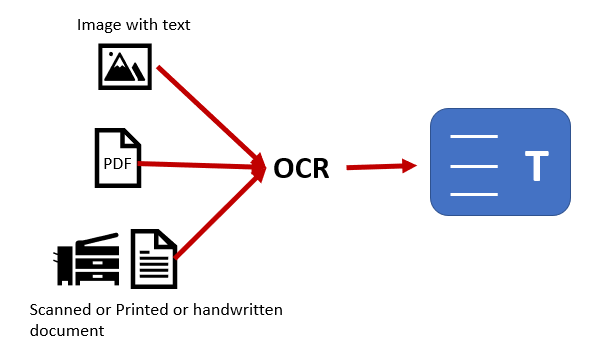
\includegraphics[width=0.45\textwidth]{Figures/Chapter 1/OCR_example.png}
    \caption{Different usages of OCR}
    \label{fig:ocrexamples}
\end{figure}

\begin{figure}[H]
   \centering
    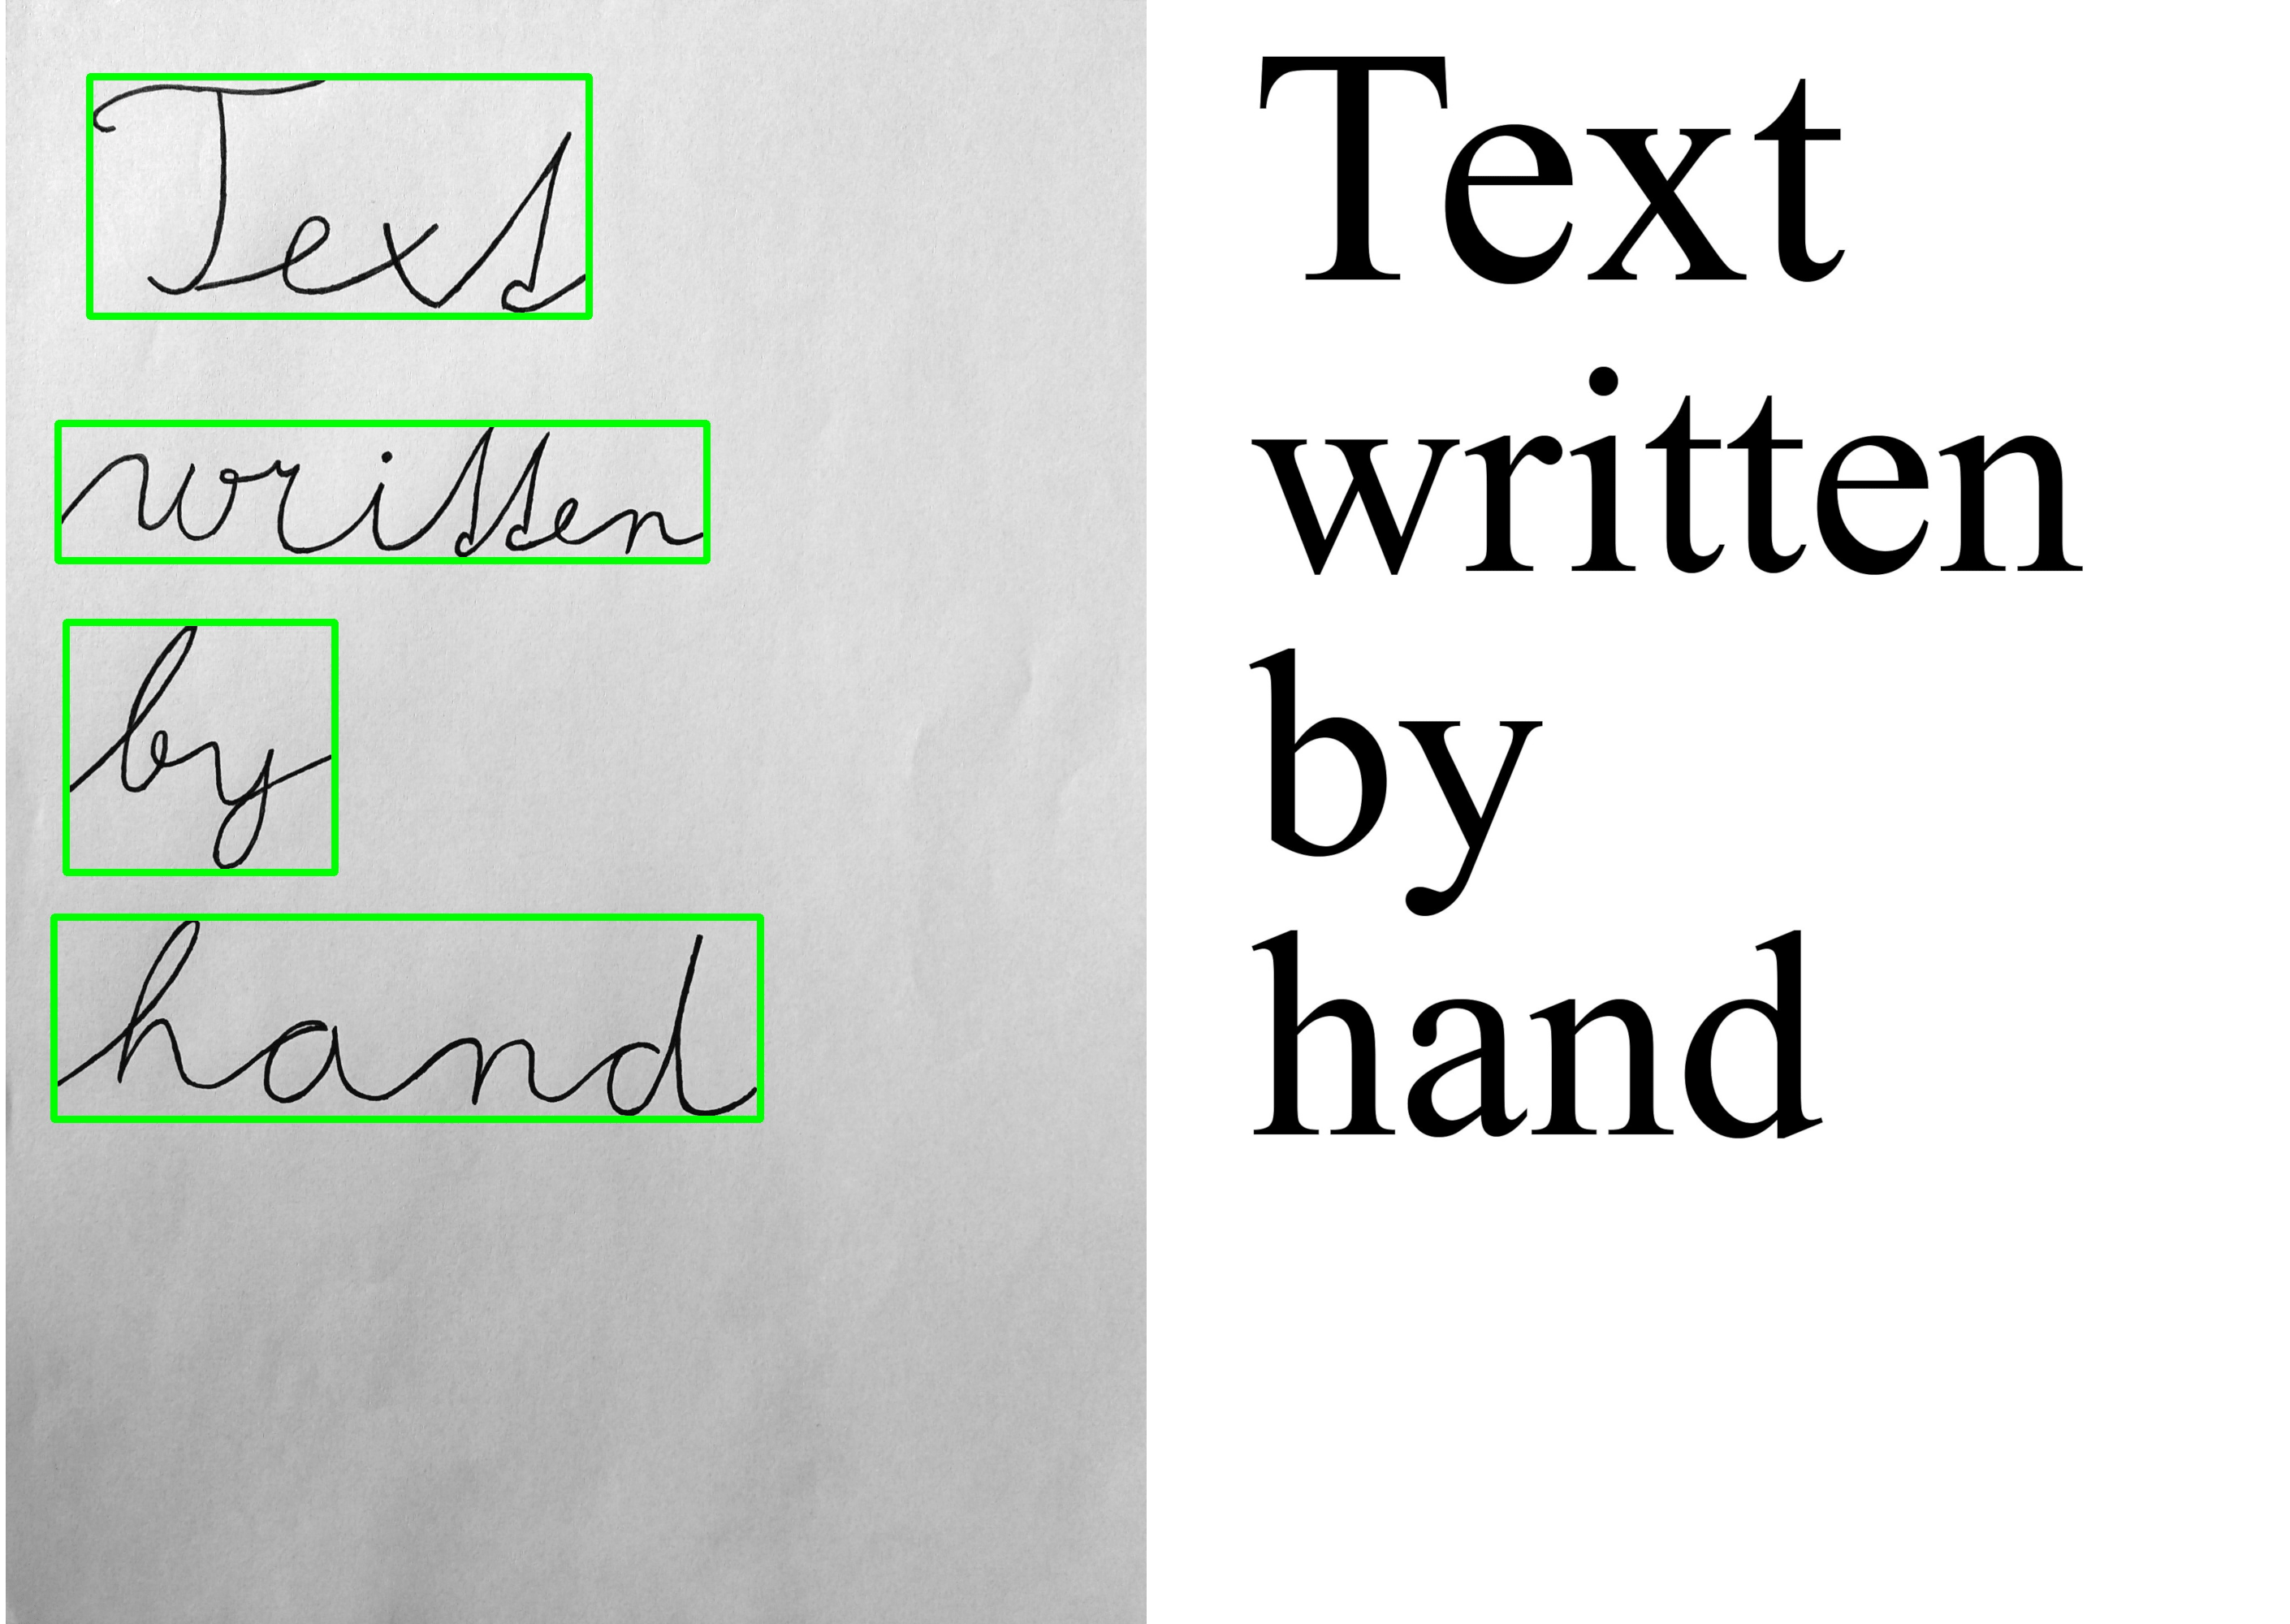
\includegraphics[height=0.2\textwidth]{Figures/Chapter 1/HTR_example.png}
    \caption{Example usage of HTR}
    \label{fig:HTRexamples}
\end{figure}


\section{Image Processing Definition}
Image processing refers to the technique of applying operations on digitalized images to enhance, analyze, and capture vital information from them. It involves different computational methods to manipulate data from images, improve visual quality, or enable interpretation by machines or humans \cite{gonzales1987digital}. Image processing is widely used in different applications such as medical imaging for analyzing X-rays, MRIs and CT scans for diagonsis and treatment planinng \cite{suzuki2017overview},  defect detection in manufactured products \cite{he2016deep} and in Optical Character Recognition which converts printed or handwritten text into digital text for document digitization \cite{smith2007overview}.%corrected

\begin{figure}[H]
    \centering
    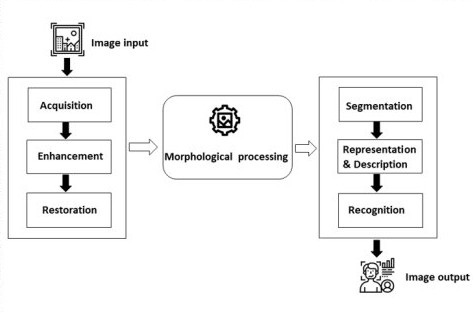
\includegraphics[width=0.8\textwidth]{Figures/Chapter 1/image_processing.jpg}
    \caption{Image processing mechanism}
    \label{fig:Imgprocessing}
\end{figure}

\subsection*{Image Processing Mechanism's Steps}
\begin{enumerate}
  \item \textbf{Acquisition of image:} The initial level begins with image pre-processing, which uses a sensor to capture the image and transform it into a usable format.

  \item \textbf{Enhancement of image:} Image enhancement is the technique of bringing out and emphasising specific interesting characteristics which are hidden in an image.

  \item \textbf{Restoration of image:} Image restoration is the process of enhancing an image's look. Picture restoration, as opposed to image augmentation, is carried out utilising specific mathematical or probabilistic models.

  \item \textbf{Colour image processing:} A variety of digital colour modelling approaches, such as HSI (Hue-Saturation-Intensity), CMY (Cyan-Magenta-Yellow), and RGB (Red-Green-Blue) etc., are used in colour picture processing.

  \item \textbf{Compression and decompression of image:} This enables adjustments to image resolution and size, whether for image reduction or restoration, depending on the situation, without lowering image quality below a desirable level. Lossy and lossless compression techniques are the two main types of image file compression that are being employed in this stage.

  \item \textbf{Morphological processing:} Digital images are processed depending on their shapes using an image processing technique known as morphological operations. The operations depend on the pixel values rather than their numerical values, and well suited for the processing of binary images. It aids in removing imperfections for structure of the image.

  \item \textbf{Segmentation, representation and description:} The segmentation process divides a picture into segments, and each segment is represented and described in such a way that it can be processed further by a computer. The image's quality and regional characteristics are covered by representation. The description's job is to extract quantitative data that helps distinguish one class of items from another.

  \item \textbf{Recognition of image:} A label is given to an object through recognition based on its description. Some of the often-employed algorithms in the process of recognising images include the Scale-invariant Feature Transform (SIFT), the Speeded Up Robust Features (SURF), and the PCA (Principal Component Analysis).
\end{enumerate} %validated

\section{Optical Character Recognition (OCR) Definition}
Optical character recognition (OCR) is the mechanical or electronic conversion of images of typed, handwritten or printed text into machine-encoded text.
It is widely used as a form of data entry from some sort of original paper data source, whether passport documents, invoices, bank statements, receipts, business cards, mail, or any number of printed records.  It is a popular technique for digitizing printed texts for electronic editing, searching, more compact storage, online display, and usage in machine processes including text-to-speech, machine translation, key data extraction, and text mining \cite{eikvil1993optical}. %validated

%\section{Open Source OCR Tools}
%There exist many OCR tools and engines in the literature. In this section, we cite a few of the popular state-of-the-art open-source OCR tools: %corrected

%\subsection{Tesseract-OCR}
%Tesseract\footnote{https://github.com/tesseract-ocr/tesseract} is a well-established OCR engine known for its flexibility and community support. Since version 4, it incorporates LSTM networks, improving recognition in challenging layouts \cite{Smith2007}. It supports custom training, allowing domain-specific fine-tuning \cite{Tzutalin2015}. However, its performance can still degrade on low-quality images or irregular fonts without proper pre-processing and training. %validated

%\subsection{Easy-OCR}
%EasyOCR\footnote{https://github.com/JaidedAI/EasyOCR} is an open-source Python library developed by Jaided AI that eases Optical Character Recognition (OCR) by extracting text from images. In addition, it supports over 80 languages including Latin, Chinese and Arabic. It uses a Convolutional Recurrent Neural Network which makes it accessible for both natural scene text and dense document text recognition tasks.\cite{JaidedAI2020}

%\subsection{TrOCR}
%TrOCR\footnote{https://github.com/microsoft/unilm/tree/master/trocr}, developed by Microsoft, employs a transformer-based architecture for end-to-end OCR. It uses a vision encoder (ViT) to process images and a language decoder (like BART) to generate text \cite{Li2021}. It has achieved state-of-the-art results on several benchmarks but requires significant computational resources for training. Its ability to fine-tune on domain-specific data makes it a strong candidate for specialized tasks like medical label reading.%validated

%\subsection{GOR}
%GOCR \footnote{https://jocr.sourceforge.net/index.html}, also known as JOCR, is a free and open-source Optical Character Recognition (OCR) program developed by Jörg Schulenburg. It transforms scanned images into editable text files. It supports various image formats such as PNM, PBM, PGM, PPM, PCX, and TGA. GOCR can work as a standalone command-line application or integrate with graphical front-ends which enhances its usability across different platforms \cite{schulenburg2004gocr}.%validated

\section{Open-Source OCR Tools/Engines}
%i added this as a replacement for the repititive text above

Several open-source OCR tools/engines have been developed to address a variety of text recognition challenges, from structured documents to complex scene text. These tools differ in architecture, accuracy, language support, and ease of customization. Notable examples include: Tesseract OCR, EasyOCR, and TrOCR, each representing a different stage in the evolution of OCR, from traditional rule-based systems to deep learning and transformer-based models.

Most of these tools/engines can be easily implemented using Python. Tesseract OCR is commonly accessed via the \texttt{pytesseract} wrapper, while EasyOCR and TrOCR are available as Python libraries and integrate well with deep learning frameworks like PyTorch. Their accessibility and open-source nature make them suitable for a wide range of academic and industrial applications. % validated


\section{Extracting text from image using OCR}
In this section, we introduce the different phases that are applied to an image to extract text from it. %added

\subsection{Pre-processing}
Pre-processing is a crucial step in Optical Character Recognition (OCR); it enhances image quality and improves the accuracy of text recognition. This step is done by preparing the input image by reducing noise, increasing contrast, and correcting distortion \cite{bieniecki2007image}. %validated
\begin{figure}[H]
    \centering
    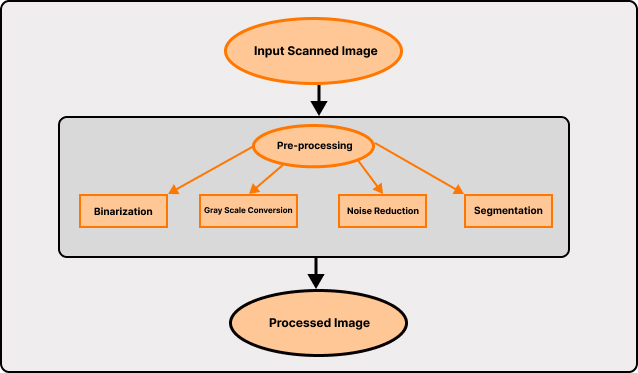
\includegraphics[width=0.90\textwidth]{Figures/Chapter 1/pre-processing.jpg}
    \caption{Image Pre-Processing procedure}
    \label{fig:imgpreprocess}
\end{figure}


Many techniques are commonly used in the pre-processing phase, all depends on the image in hands:


\subsubsection{Binarization (Thresholding)}
Binarization converts a grayscale image into a black-and-white image, which makes the text stand out from the background. Common methods include Otsu's thresholding and adaptive thresholding which dunamically adjust to lighting variations.%validated

\subsubsection{Gray Scale Conversion}
Gray Scale Conversion transforms a color image into a grayscale image (black-to-white intensity) to simplify data processing which helps with reducing computational complexity and improves contrast for character recognition.%validated
    

\begin{figure}[H]
    \centering
    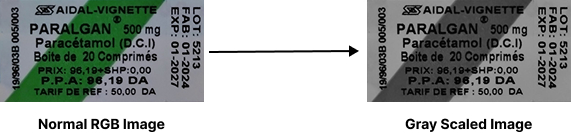
\includegraphics[width=0.90\textwidth]{Figures/Chapter 1/Gray_scale.jpg}
    \caption{Gray Scale example on Medical Labels}
    \label{fig:grayscale}
\end{figure}
%\end{comment}
%\begin{comment}

\subsubsection{Noise Reduction}
Noise Reduction removes unwanted artifacts such as speckles, dust, or blurs that might interfere with OCR. Noise reduction techniques such as Gaussian Blurring and median filtering are more commonly used to smooth images while preserving text structure. %validated

\subsubsection{Segmentation (Text Line and Character Segmentation)}
Segmentation splits words into individual characters or lines to make recognition more effective. It can be applied to lines of text, individual words, or small characters and it can be helpful when applying OCR since it isolates all the other variables and focuses only on the input text.%validated

\subsection{Text Detection}
Text Detection identifies and localizes text regions within an image before performing text recognition. This step is important when dealing with complex backgrounds or varying fonts, as improperly detected text regions can lead to misinterpretation by the OCR engine. Different types of methods are used for this phase: %corrected

\subsubsection{Traditional Text Detection Methods}
Early OCR systems relied on classical computer vision techniques to detect text regions. It involves analyzing pixel intensity variations and identifying patterns that resemble textual structures. Some common approaches include edge detection, Contour Analysis and Connected Component Analysis \cite{gllavata2003robust}. %validatedn, here cite a paper or two using this kind of method (you can use a paper cited before in other sections if they use it) 

\subsubsection{Deep Learning-Based Text Detection Methods}
The Advancements in deep learning have significantly improved text detection accuracy, especially in natural scene images. Text detection models like YOLO (You Only Look Once) \cite{redmon2016you}, EAST (Efficient and Accurate Scene Text Detector)  \cite{zhou2017east}, CRAFT (Region Awareness for Text detection)  \cite{baek2019character}, DOCTR (Document Text Recognition) \cite{mindee2021doctr}, combine the traditional techniques for structured documents and deep learning models for unstructured scenes in order to achieve high accuracy accros various applications\cite{zhou2017east,
baek2019character}.%validatedn, here cite a paper or two using this kind of methods (you can use paper cited before in other sections if they use it)

\subsection{Text Recognition}
Text recognition is the core component of extracting text from images using OCR. It is responsible for converting detection regions into machine-readable characters, and it focuses on interpreting the textual content within the localized bounding boxes from the text detection step.%validated

\subsubsection{Traditional Text Recognition Methods}
Earlier OCR systems relied on handcrafted features and rule-based methods to recognize characters; these approaches were effective for structured documents but struggled with other variations. Some of the key traditional methods are Template Matching and Feature Extraction \cite{casey1996survey}. %validatedn, here cite a paper or two using this kind of methods (you can use paper cited before in other sections if they use it)  


\subsubsection{Deep Learning-Based Text Recognition Methods}
With the advancements in Deep Learning, Text recognition systems are now much more accurate and dependable when handling complicated scenes, different fonts, or noisy backgroundsUnlike traditional Text Recognition, Deep Learning-based methods can learn directly from large datasets, allowing them to be adaptable to any type of document or text.
One of the most widely used architectures is the Convolutional Recurrent Neural Network (CRNN)\cite{shi2017crnn} which combines the Convolutional Neural Networks ability for feature extraction and Recurrent Neural Networks for sequence modelling, and more recently, Transformer-based models like TrOCR use the the Vision Transformer (ViT)\cite{dosovitskiy2020image} mechanism to extract feature and their self-attention mechanisms allow them to focus on relevant parts of the image making them particularly powerful for handling complex layouts or irregular handwriting \cite{lecun1998gradient, graves2009offline}. %validatedn, here cite a paper or two using this kind of methods (you can use paper cited before in other sections if they use it)


    
\subsection{Post-processing}
After text has been recognized by the OCR engine, a Post-Processing step is often applied to ensure higher accuracy, which is important when dealing with noisy images or domain-sepcific languages.

\subsubsection{Text Correction}
Text correction is a common first step where spell checking algorithms are deployed to fix misrecognized words. For example, if the OCR output was "med1cation", post processing might correct it to "medication" based on context \cite{soper2021bart}.%validatedn, here cite a paper or two using this kinf of methods (you can use paper cited before in other sections if they use it)

\subsubsection{Normalization}
Normalization includes converting text to a consistent case (e.g., all lowercase), removing non-alphanumeric symbols, and standardizing formats for things like dates or units \cite{duong2020unsupervised}.%validatedn, here cite a paper or two using this kinf of methods (you can use paper cited before in other sections if they use it)

\section{Case Study: Information detection and recognition from medical labels - Algeria}
This section describes our case study, which is about detecting and recognizing the text from the medical labels represented in images.

\subsection{What is a medical label?}
A medical label is a small sticker that is found on medicine boxes or bottles. It serves as a vital resource in the healthcare industry as it provides crucial information about the medicines, such as the dosage, price, expiration date, and whether or not they are covered by insurance. By providing this information clearly and accurately, medical labels help ensure patient safety, proper medication usage, and easier access to necessary treatments.%validated

\subsection{Medical labels use in Algeria}

In Algeria, medical labels serve as an important communication tool between pharmacists and patients. They provide essential information such as the medication's name, dosage instructions, expiration date, price, and insurance coverage status. Aside from patient communication, medical labels also play a vital role in the commercial and administrative operations of pharmacies. Commercially, pharmacists use label information to set prices, manage inventory, and maintain sales records. Administratively, labels help ensure regulatory compliance, proper storage conditions, and accurate tracking of dispensed medications. %validated

\subsection{Types of medical labels}
In Algeria, most medical labels are split into three types of stickers:
\begin{itemize}
    \item \textbf{Green Medical Labels:} Represents the Refundable medications.
    \item \textbf{Red Medical Labels:} Represents the non-Refundable medications.
    \item \textbf{White Medical Labels:} Represents the non-Refundable vitamins or supplements.
\end{itemize}
   

\begin{figure}[H]
    \centering
    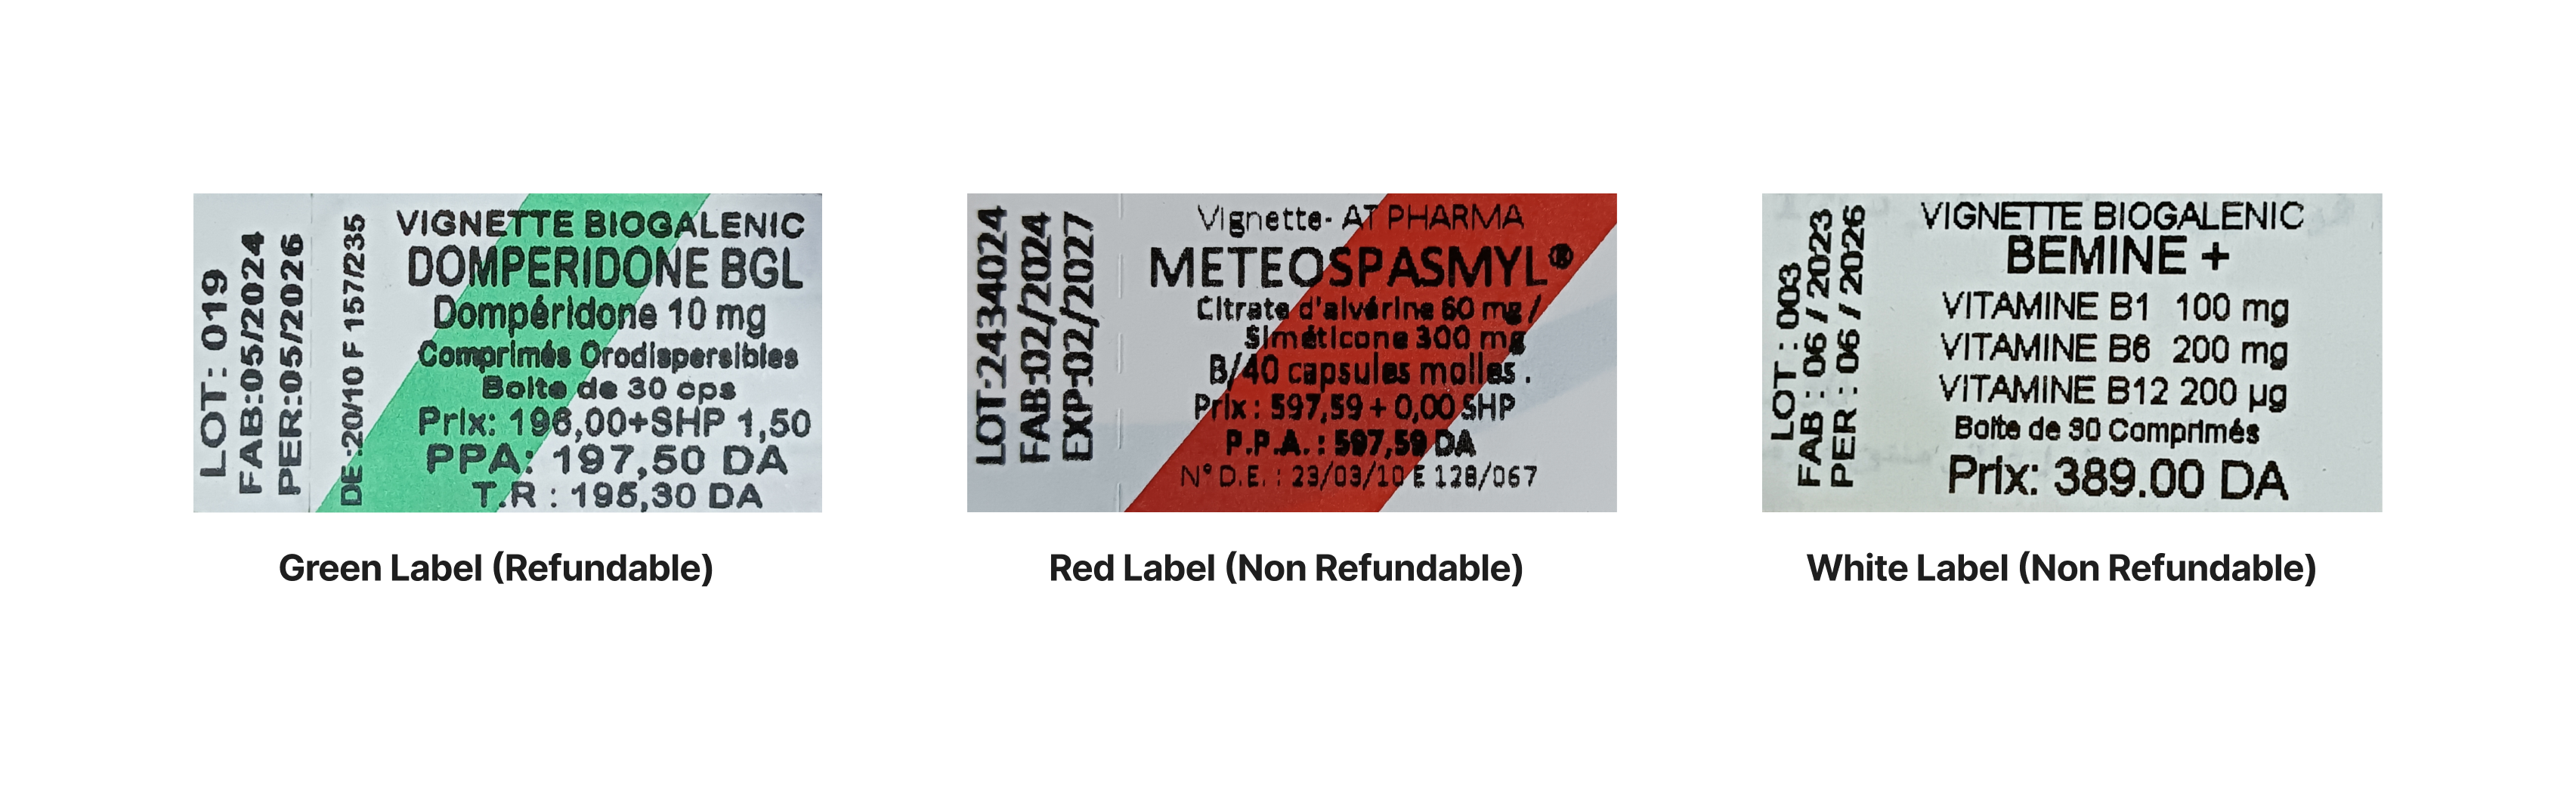
\includegraphics[width=\textwidth]{Figures/Chapter 1/labels_types.png}
    \caption{Types of Medical Labels}
    \label{fig:typesofmedicallabels}
\end{figure}

\subsection{Medical label information content}
All 3 types of medical labels contain important information that are useful to the customers, patients, and pharmacists. The information is like the following:

\begin{enumerate}
    \item Name of the medication 
    \item Dosage
    \item Dosage format (Grams, Miligrams)
    \item \textbf{PPA:} Algerian Public Price (Prix Public Algerien in French) 
    \item \textbf{TR:} The price in the case of purchasing using a reimbursement card "Shiffa"
    \item \textbf{SHP:} Pharmacist Honorary Supplement (Supplément Honorifique de Pharmacien in french)
    \item \textbf{FAB:} Date of manufacture
    \item \textbf{EXP:} Expiration Date
    \item \textbf{LOT:} The batch number
\end{enumerate}

\section{Medical label information processing in Algeria}
In this digitized era, most information is now processed automatically and streamlined for the sake of time, convenience, and accuracy. However, Algerian pharmacies are not fully leveraging the potential of medication labels in a digital sense. They merely use them for basic medicine identification and to check the reimbursement status with insurance entities such as CNAS (Caisse Nationale des Assurances Sociales) and CASNOS (Caisse Nationale de Sécurité Sociale des Non-Salariés). The process of submitting medication information to CNAS still relies heavily on manual methods: medication stickers are attached to the back of prescription sheets, after which a worker manually verifies the information on the medication labels by comparing it with the details in the delivery note (le bordereau).

\section{Conclusion}
In this chapter, we presented an introductory overview of some general concepts of Text Recognition for an efficient text recognition system. We discussed its evolution from traditional techniques to deep learning-based methods, and outlined the key steps involved in the OCR pipeline. Several widely used open-source OCR tools/engines were introduced, along with the roles of image pre-processing, text detection, recognition, and post-processing in text recognition systems, along with a few commonly used methods and techniques.
...
Additionally, we examined a case study centered on the detection and recognition of medical label information in the Algerian context. This study highlighted the significance of medical labels as carriers of essential pharmaceutical information and the need for automated OCR-based solutions to improve efficiency, accuracy, and integration with healthcare administrative systems.

%\end{comment}






